\chapter{Les Houches Lecture Notes on Tensor Networks}
\section{Synopsis}
These lecture notes are based on a series of five lectures taught by Frank Verstraete at the 2025 Les Houches school on \emph{Exact Solvability and Quantum Information}. They cover a variety of topics in the field of tensor networks, with an emphasis on the concept of the MPS manifold, MPO symmetries, integrability and dualities.
\section{Reference}
\textit{Les Houches Lecture Notes on Tensor Networks}, \par\noindent
\textbf{B. Vancraeynest-De Cuiper}, W. Wiesiolek, F. Verstraete \par\noindent
%\href{https:/doi.org/10.21468/SciPostPhys.19.2.054}{SciPost Phys. \textbf{19}, 054 (2025)},
\href{https://doi.org/10.48550/arXiv.2512.24390}{arXiv:2512.24390}
\section{Contributions of the author}
I wrote the majority of the manuscript, whose content closely follows that of the lectures on which it is based. Apart from some aspects of the exposition, the content is due to the lecturer.
%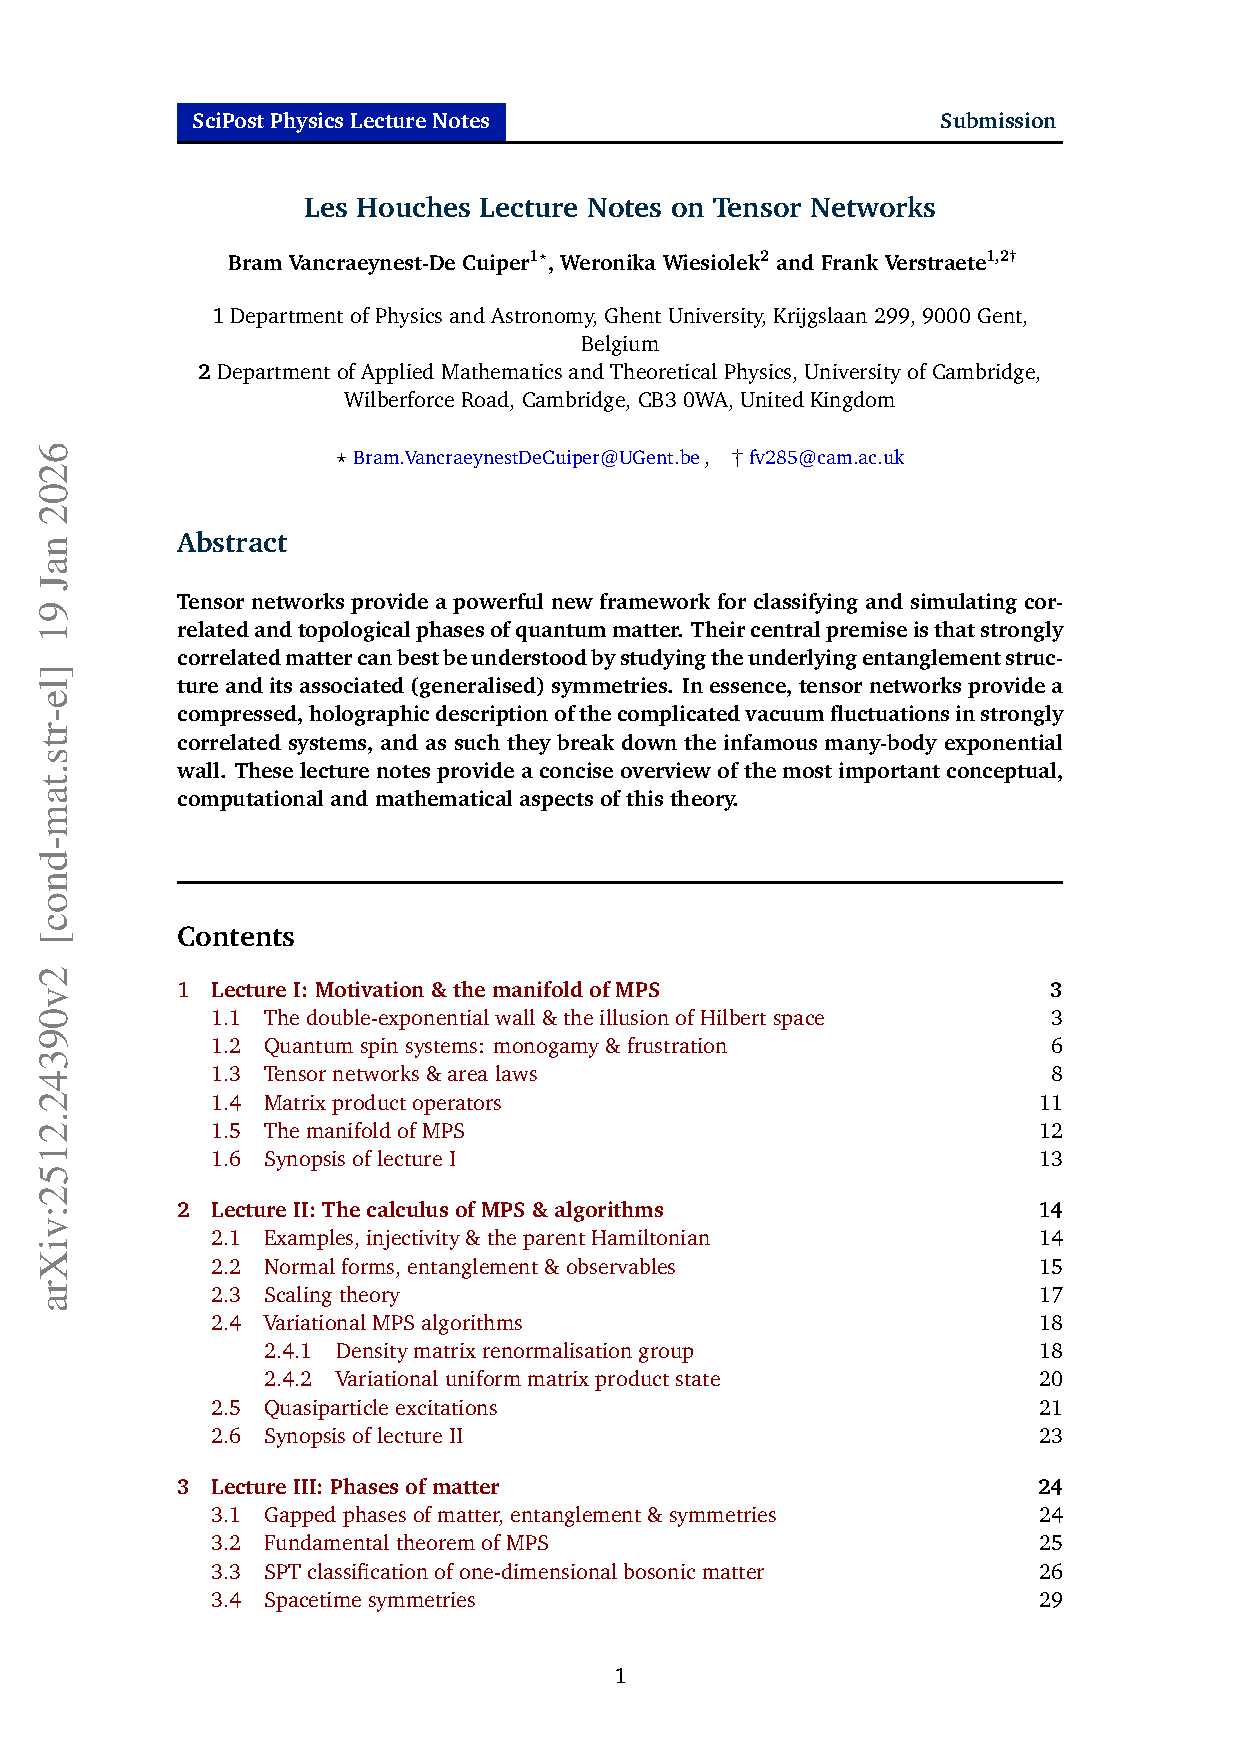
\includepdf[pages=1-4, trim=1.5cm 1.5cm 1.5cm 1.5cm, offset=-4mm 0mm, clip=true, frame=false, noautoscale=true, width=1.04\headwidth, pagecommand={}]{papers/lecture_notes}
%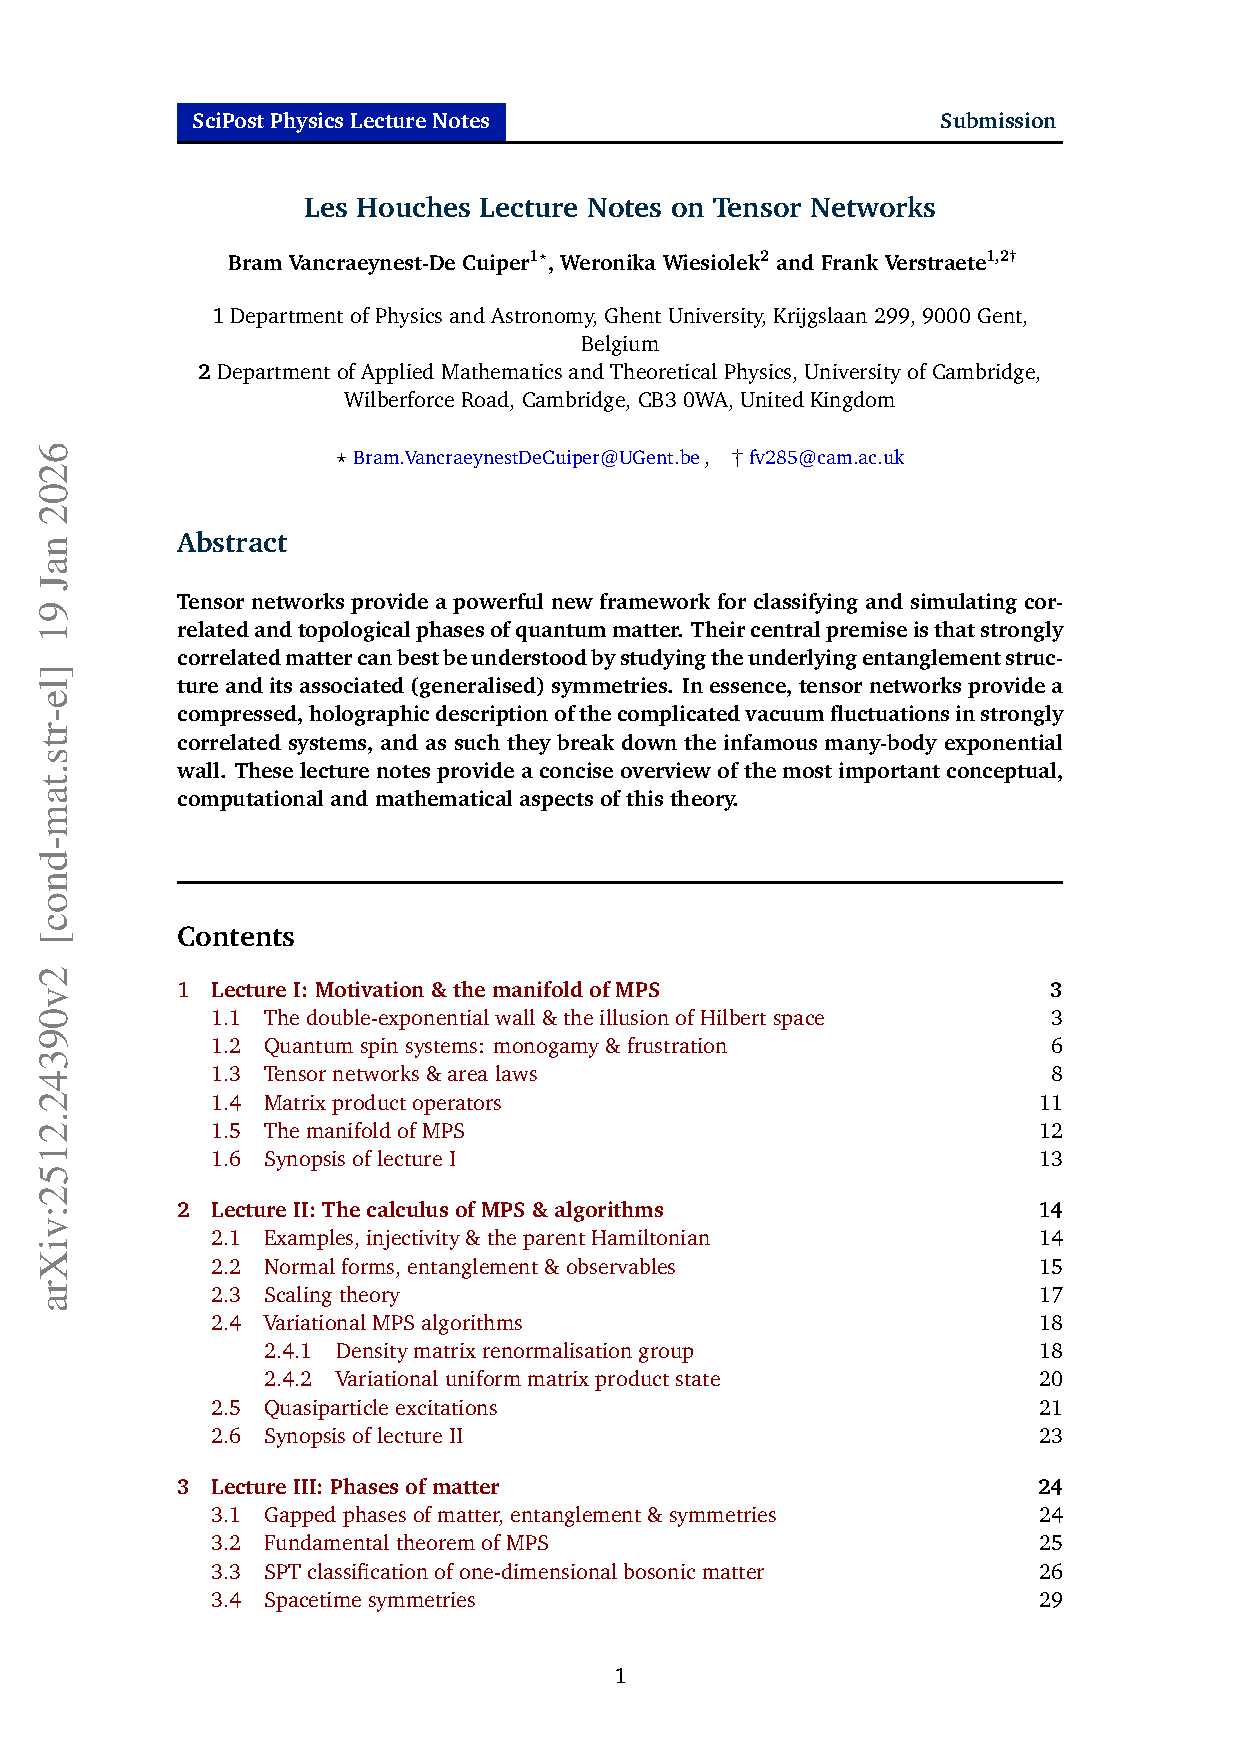
\includepdf[pages=-, trim=1.3cm 1.8cm 1.3cm 0cm, offset=-4mm 7mm, clip=true, frame=false, noautoscale=true, width=1.08\headwidth, pagecommand={}]{papers/lecture_notes}
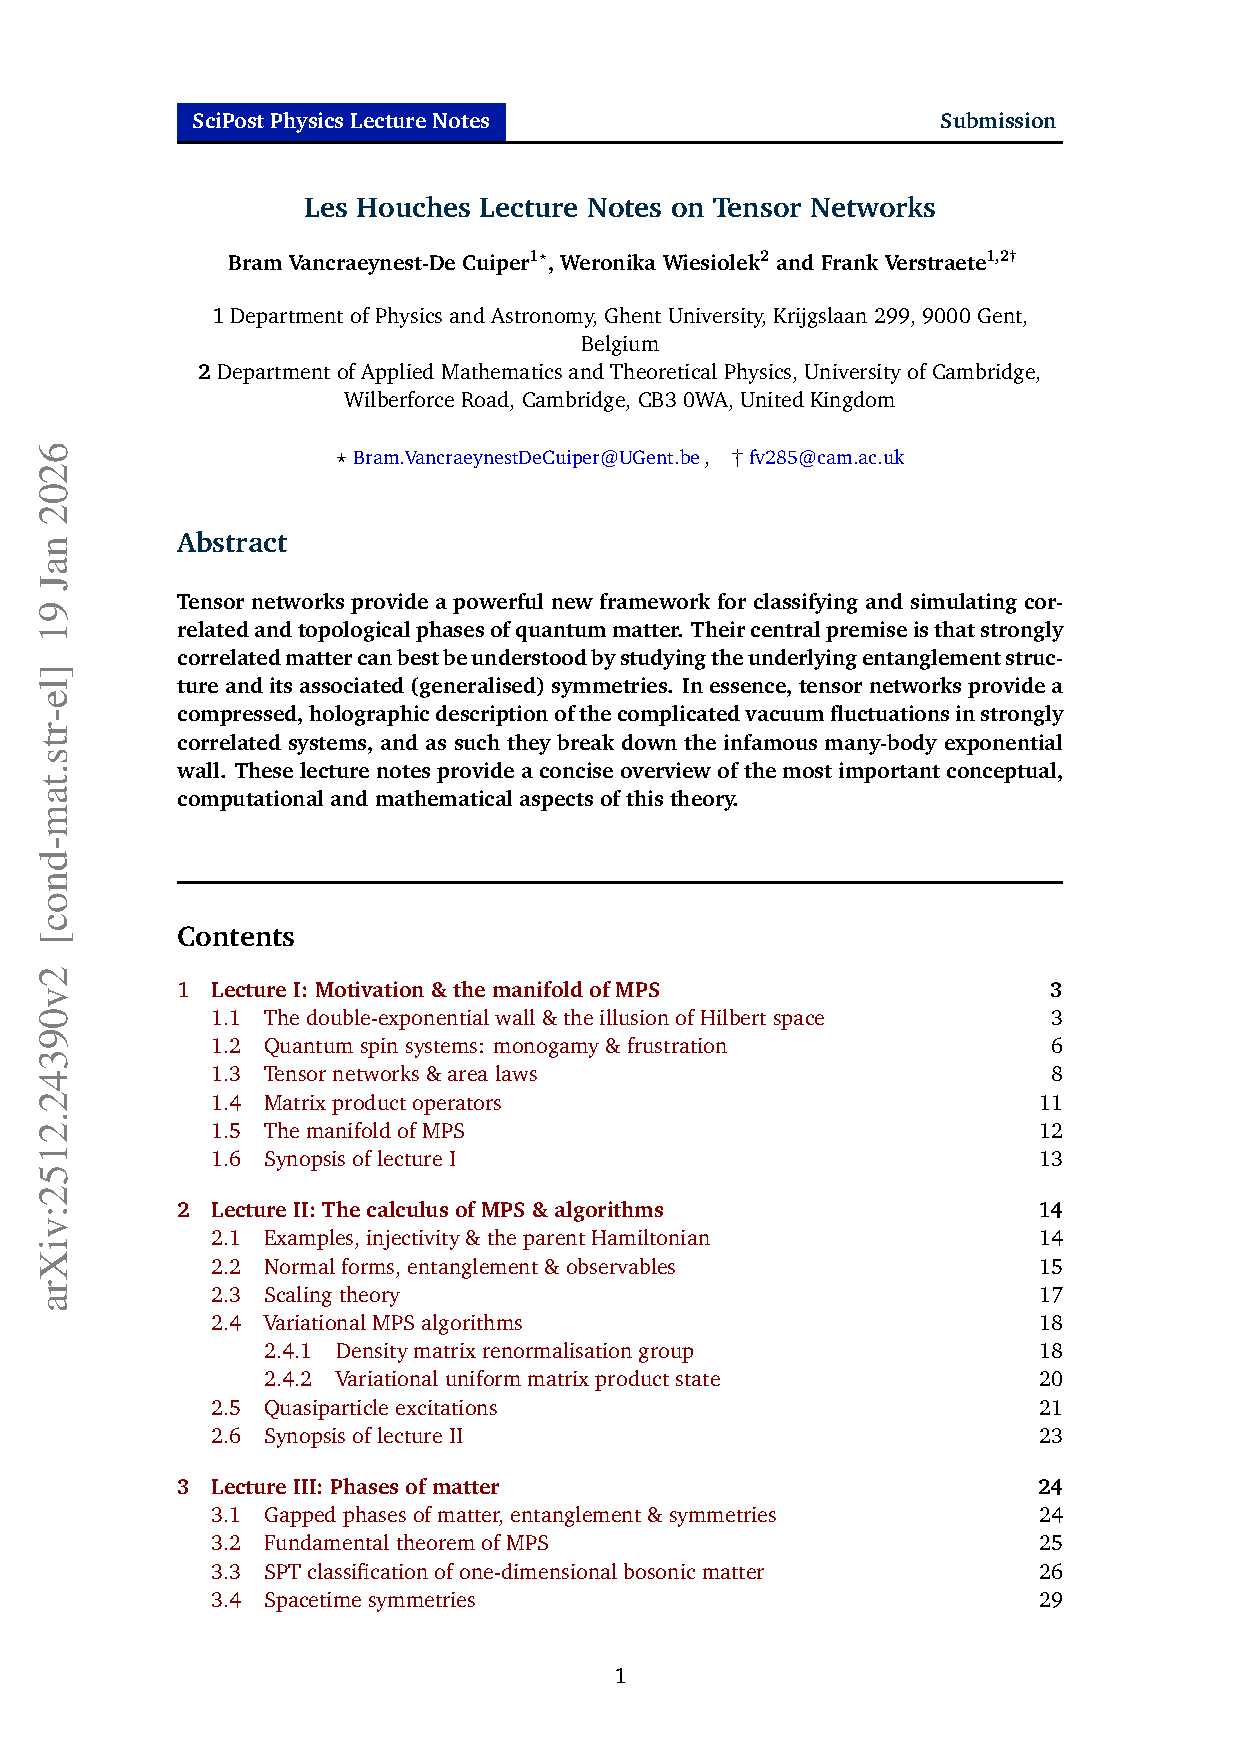
\includepdf[pages=-,
trim=25mm 20.54mm 25mm 18mm, clip=true,
noautoscale=true, height=\textheight,
offset=-0.65mm 4mm,
pagecommand={\thispagestyle{publication}}]{papers/lecture_notes}